\documentclass[../../main.tex]{subfiles}

\graphicspath{{../../fig/}}
\setcounter{section}{0}

\begin{document}

\chapter{宇宙マイクロ波背景放射(CMB)}
宇宙マイクロ波背景放射(Cosmic Microwave Background: CMB)とは、宇宙の創生から38万年後に物質から脱結合した光子のことであり、我々が観測できる最古の光である。
その発見はペンジアスとウィルソンによって1965年に行われ\cite{1965ApJ...142..419P}、
その後Cosmic Background Explorer(COBE)衛星により強度の周波数依存性(スペクトル)が測定された\cite{1996ApJ...473..576F}。
測定されたスペクトルは温度が$\SI{2.725}{K}$の黒体輻射のスペクトルと一致し(図\ref{fig:cobe})、CMBがほとんど一様等方な強度を持つことも確認された。
これらの事実によりCMBはビッグバン宇宙モデルを支持する強力な証拠となった。
こうして現代の宇宙論の基礎を築き、発展させてきたCMBは、現在ではその偏光情報からインフレーション宇宙論の証拠を探ることができると期待されている。
本章では、はじめに現在の標準的な宇宙モデルである$\Lambda\mathrm{CDM}$モデルについて述べ、次いでインフレーション宇宙論について述べる。
その後、CMB偏光について述べる。
\begin{figure}[H]
    \centering
    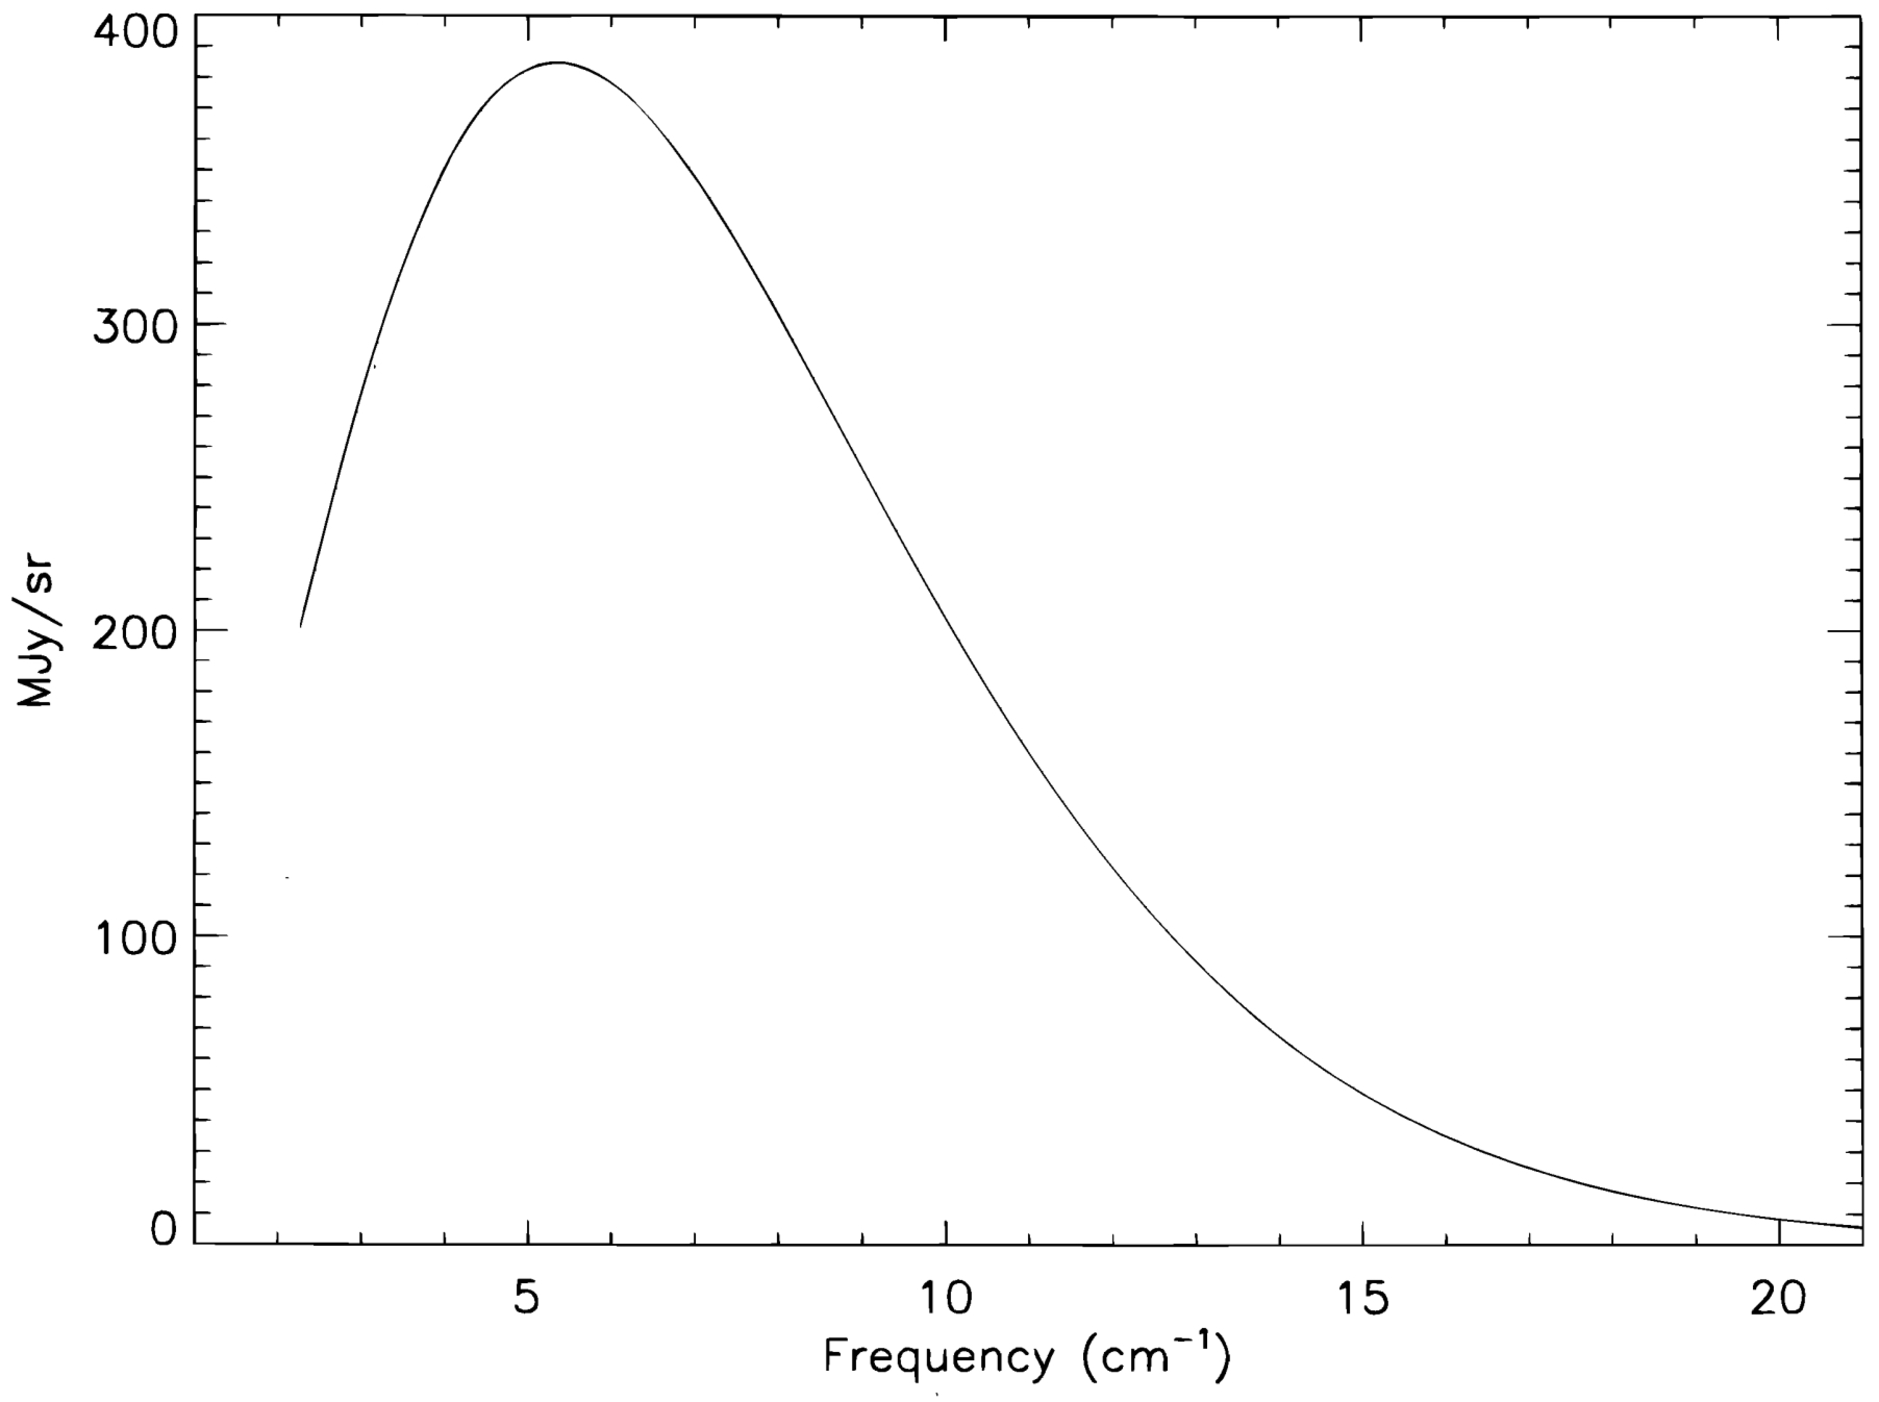
\includegraphics[width=0.6\textwidth]{intro/cobe.pdf}
    \caption{COBE衛星によるCMBのスペクトル測定値を黒体輻射のスペクトルでfittingした結果。}
    \label{fig:cobe}
\end{figure}

\section{$\Lambda\mathrm{CDM}$モデル}
現在の標準的な宇宙モデルである$\Lambda\mathrm{CDM}$モデルについて述べる。
まず、Einstein方程式は、計量テンソル$g_{\mu\nu}$、Einsteinテンソル$G_{\mu\nu}$とエネルギー運動量テンソル$T_{\mu\nu}$を用いて
\begin{equation}
    \label{eq:einstein}
    G_{\mu\nu}+\Lambda g_{\mu\nu}=8\pi GT_{\mu\nu}
\end{equation}
とかける。ここで、$G$は重力定数、$\Lambda$は宇宙定数である。また、自然単位系を採用した。
一様等方な宇宙では、その計量はフリードマン・ルメートル・ロバートソン・ウォーカー計量
\begin{equation}
    \label{eq:rwmetric}
    ds^2=-dt^2+a^2(t)\qty[\frac{dr^2}{1-Kr^2}+r^2d\Omega^2]
\end{equation}
で記述される。ここで、$a(t)$はスケールファクター、$K$は宇宙の曲率を表す。
また、宇宙の物質が完全流体であることを仮定すると、エネルギー運動量テンソルを
\begin{equation}
    \label{eq:emtensor}
    T_{\mu\nu}=\mqty(-\rho&0&0&0\\0&P&0&0\\0&0&P&0\\0&0&0&P)
\end{equation}
と表すことができる。ここで、$\rho$はエネルギー密度、$P$は圧力である。
エネルギー運動量テンソルを用いてエネルギー保存則を考えると
\begin{equation}
    \label{eq:energyconservation}
    \dot{\rho}+3\dfrac{\dot{a}}{a}(\rho+P)=0
\end{equation}
を得る。
式\eqref{eq:rwmetric}、式\eqref{eq:emtensor}を式\eqref{eq:einstein}に代入し、$(0,\,0)$に注目すると
\begin{align}
    \label{eq:friedmann}
    H^2:=\qty(\dfrac{\dot{a}}{a})^2 &= \dfrac{8\pi G}{3}\rho+\dfrac{\Lambda}{3}-\dfrac{K}{a^2}
\end{align}
を得る。これをフリードマン方程式と呼ぶ。$H:=\dot{a}/a$はハッブル定数である。
これまでのCMBの観測から、宇宙が平坦であると考えられている\cite{Bennett_2003}ため、以下では$K=0$とする。
$\Lambda\mathrm{CDM}$モデルでは、宇宙を構成する成分として、物質、放射、ダークエネルギーが存在すると考え、
エネルギー密度$\rho$は各成分のエネルギー密度の和として表される。すなわち、フリードマン方程式は
\begin{equation}
    \label{eq:friedmann2}
    H^2=H_0^2\qty(\Omega_m(1+z)^3+\Omega_r(1+z)^4+\Omega_{\Lambda})
\end{equation}
と書ける。ここで、$\rho_m$は物質のエネルギー密度、$\rho_r$は放射のエネルギー密度、$\rho_{\Lambda}$はダークエネルギーのエネルギー密度である。

\section{インフレーション宇宙論}

\section{CMB偏光モード}
\section{本論文の構成}

\end{document}